\hypertarget{day-2---ux7f16ux5199-web-app-ux9aa8ux67b6}{%
\subsection{Day 2 - 编写 Web App
骨架}\label{day-2---ux7f16ux5199-web-app-ux9aa8ux67b6}}

由于我们的 Web App 建立在 asyncio 的基础上,因此用 aiohttp
写一个基本的\texttt{app.py}:

\begin{pythoncode}
import logging; logging.basicConfig(level=logging.INFO)

import asyncio, os, json, time
from datetime import datetime

from aiohttp import web

def index(request):
    return web.Response(body=b'<h1>Awesome</h1>')

@asyncio.coroutine
def init(loop):
    app = web.Application(loop=loop)
    app.router.add_route('GET', '/', index)
    srv = yield from loop.create_server(app.make_handler(), '127.0.0.1', 9000)
    logging.info('server started at http://127.0.0.1:9000...')
    return srv

loop = asyncio.get_event_loop()
loop.run_until_complete(init(loop))
loop.run_forever()
\end{pythoncode}

运行\texttt{python\ app.py},Web App 将在\texttt{9000}端口监听 HTTP
请求,并且对首页\texttt{/}进行响应:

\begin{pythoncode}
$ python3 app.py
INFO:root:server started at http:
\end{pythoncode}

这里我们简单地返回一个\texttt{Awesome}字符串,在浏览器中可以看到效果:

 
 \begin{figure}[htp]
	\centering
	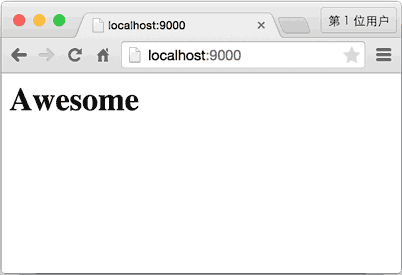
\includegraphics[width=0.6\linewidth]{fig/1019401123918240l.png}
\end{figure}


这说明我们的 Web App 骨架已经搭好了,可以进一步往里面添加更多的东西。

\hypertarget{ux53c2ux8003ux6e90ux7801}{%
\subsubsection{参考源码}\label{ux53c2ux8003ux6e90ux7801}}

\href{https://github.com/michaelliao/awesome-python3-webapp/tree/day-02}{day-02}

